\documentclass[11pt]{article}
\usepackage[margin=1in]{geometry}
\usepackage{amsmath,amssymb}
\usepackage{booktabs}
\usepackage{graphicx}
\usepackage{hyperref}
\usepackage{float}

\newcommand{\E}{\mathbb{E}}
\newcommand{\R}{\mathbb{R}}

\title{Data 37711 Homework 2 --- Problem 3\\
\large Random Kitchen Sinks vs.\ a one-hidden-layer MLP}
\author{Yiwen Chen}
\date{}

\begin{document}
\maketitle

The code is in \texttt{problem3.py}. It uses the provided \texttt{dataloader.py} and
\texttt{plotting.py}; \texttt{models.py} was used as a template, and both models are implemented
in the script. The data are 600 training points, 200 validation points, and 200 unlabelled test
points, with $(x_1,x_2)\in[-3,3]^2$. Predicting the training mean gives a validation MSE of
$2.397$, which is the baseline every model should beat by a wide margin.

%==========================================================================
\section*{(a) Data visualization}

\begin{figure}[H]\centering
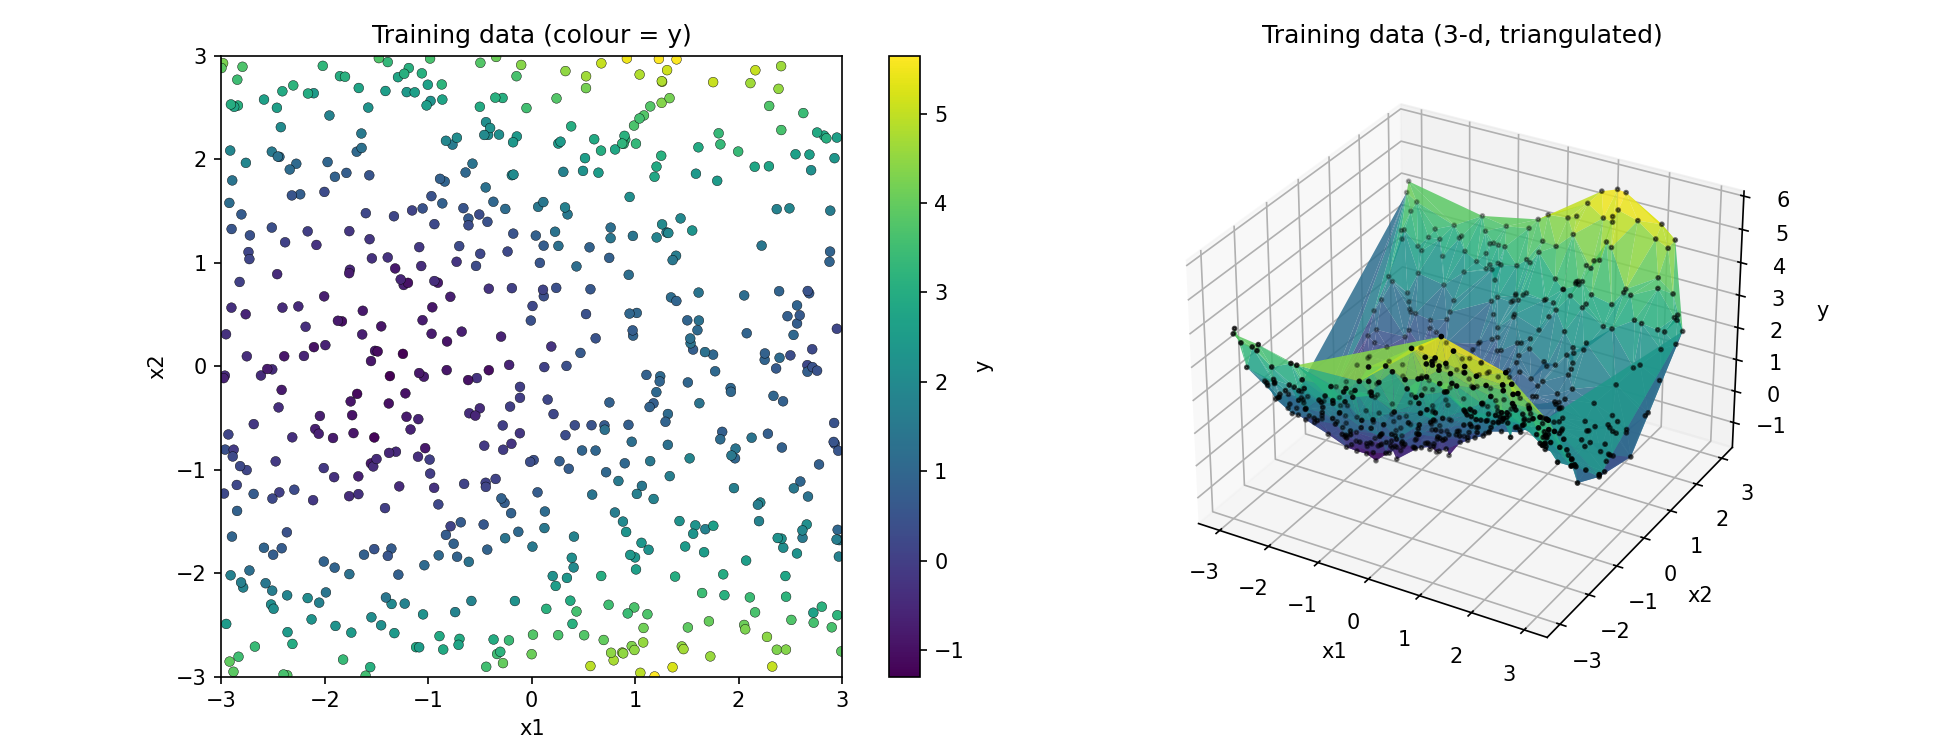
\includegraphics[width=\textwidth]{problem3_data.png}
\caption{Training data. Left: points coloured by $y$. Right: a 3-d view (Delaunay-triangulated
surface through the training points).}
\label{fig:data}
\end{figure}

The response surface is smooth and has a clear structure:
\begin{itemize}
\item Along $x_2$ it is roughly \textbf{symmetric and U-shaped}. $y$ is smallest near $x_2=0$ and
grows towards $x_2=\pm3$.
\item Along $x_1$ it \textbf{oscillates once}. There is a valley around $x_1\approx-1.5$, where the
minimum $y\approx-1$ is reached near $(x_1,x_2)\approx(-\pi/2,0)$, and a ridge around
$x_1\approx+1.5$, where the largest values $y\approx5.5$ occur in the corners
$(\approx\pi/2,\pm3)$.
\end{itemize}
This looks like $y\approx\sin(x_1)+c\,x_2^2$ plus noise. An exploratory least-squares fit of
$y=\beta_0+\beta_1\sin x_1+\beta_2x_2^2$ on the training set gives
$(\beta_0,\beta_1,\beta_2)=(-0.01,\,1.01,\,0.50)$ and a \emph{validation} MSE of $0.0353$. So the
data are close to $y=\sin(x_1)+\tfrac12x_2^2+\varepsilon$ with
$\operatorname{Var}(\varepsilon)\approx0.034$. I use $0.035$ as a rough \emph{noise floor} for the
validation MSE when judging the flexible models below. They are not given this functional form.

%==========================================================================
\section*{(b) Random Kitchen Sinks with ridge regression}

\paragraph{Model.} For $j=1,\dots,h$ draw $w_j\sim\mathcal N(0,I_2/\sigma^2)$ and
$b_j\sim\mathcal U[0,2\pi]$, and map
\[
 z(x)=\bigl(\sin(w_1^\top x+b_1),\cos(w_1^\top x+b_1),\dots,\sin(w_h^\top x+b_h),\cos(w_h^\top x+b_h)\bigr)^\top\in\R^{D},
 \qquad D=2h .
\]
On top of these random features I fit ridge regression with an unpenalized intercept,
\[
 \min_{\beta_0,\beta}\;\frac1n\sum_{i=1}^n\bigl(y_i-\beta_0-\beta^\top z(x_i)\bigr)^2+\lambda\lVert\beta\rVert_2^2 .
\]
Centring $Z$ and $y$ removes $\beta_0$. Setting the gradient to zero gives the closed form
\[
 \hat\beta=\bigl(Z_c^\top Z_c+n\lambda I_D\bigr)^{-1}Z_c^\top y_c,\qquad
 \hat\beta_0=\bar y-\bar z^\top\hat\beta ,
\]
where $Z_c=Z-\mathbf 1\bar z^\top$ and $y_c=y-\bar y\mathbf 1$. The problem is strictly convex,
so this is the unique global optimum. No iterative training is needed.

\paragraph{Why $\sigma$ matters (kernel view).} Using $\sin a\sin b+\cos a\cos b=\cos(a-b)$,
\[
 \frac1h\,z(x)^\top z(x')
 =\frac1h\sum_{j=1}^h\cos\bigl(w_j^\top(x-x')\bigr)
 \xrightarrow[h\to\infty]{\text{a.s.}}
 \E_w\bigl[\cos(w^\top\delta)\bigr]
 =\exp\!\Bigl(-\frac{\lVert x-x'\rVert^2}{2\sigma^2}\Bigr),
 \qquad\delta=x-x',
\]
by the law of large numbers ($w_1,\dots,w_h$ are i.i.d.\ and $|\cos|\le1$). Here
$\E[\cos(w^\top\delta)]$ is the characteristic function of $\mathcal N(0,I/\sigma^2)$
evaluated at $\delta$. (The phases $b_j$ cancel when sin/cos pairs are used.) RKS with ridge is
therefore a Monte-Carlo approximation of \textbf{Gaussian-kernel ridge regression with bandwidth
$\sigma$}. A small $\sigma$ means high-frequency features and a very wiggly function class, and a
large $\sigma$ means low-frequency features and a very smooth function class. So $\sigma$ directly
controls the bias--variance trade-off. I therefore sweep $\sigma$.

\paragraph{Sweep.} I fix $D=1000$ ($h=500$) and $\lambda=10^{-3}$, and vary $\sigma$ over 16
log-spaced values in $[0.05,10]$. Each value is repeated over 5 random draws of $(w_j,b_j)$, and I
report mean $\pm$ sd.

\begin{figure}[H]\centering
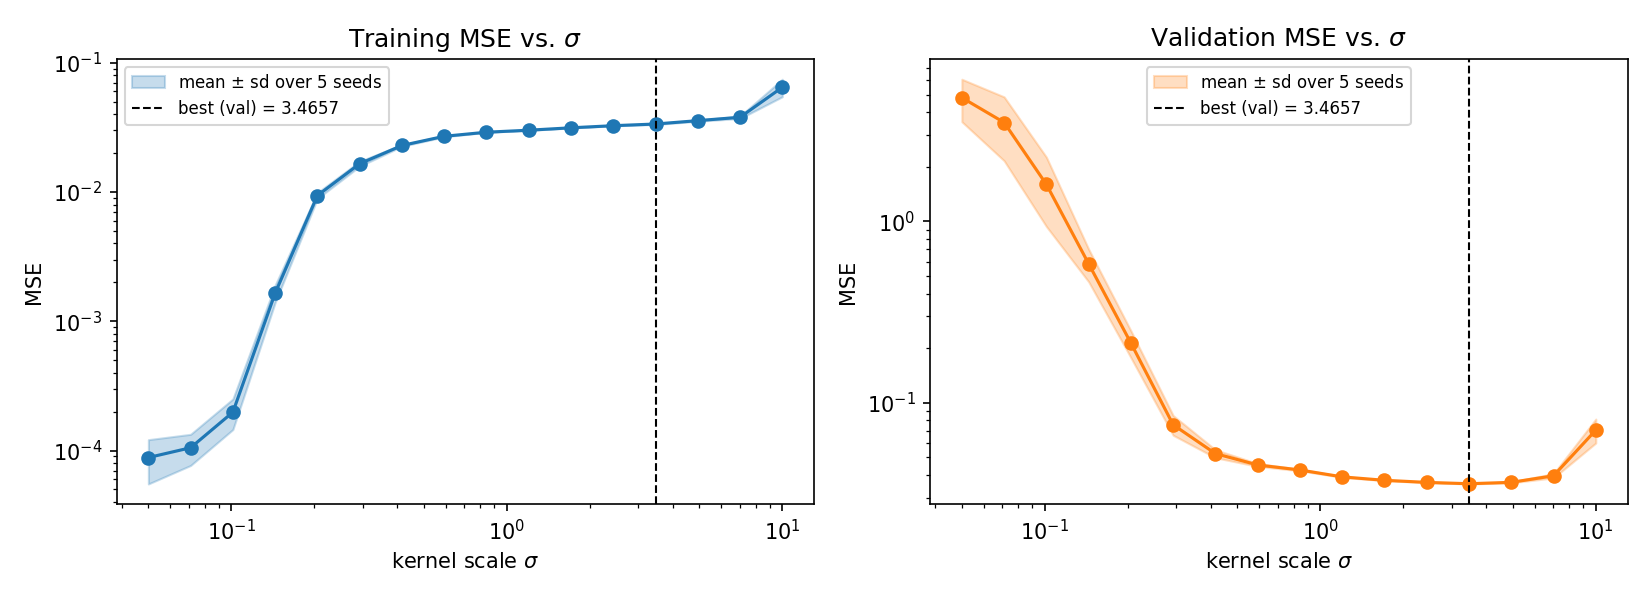
\includegraphics[width=\textwidth]{problem3_rks_sweep.png}
\caption{RKS: training (left) and validation (right) MSE vs.\ kernel scale $\sigma$
($D=1000$, $\lambda=10^{-3}$; mean $\pm$ sd over 5 seeds; log axes).}
\label{fig:rks}
\end{figure}

\begin{table}[H]\centering\small
\begin{tabular}{lcccccccc}
\toprule
$\sigma$ & 0.05 & 0.10 & 0.21 & 0.42 & 0.84 & 1.71 & \textbf{3.47} & 10.0\\
\midrule
train MSE & 0.0001 & 0.0002 & 0.0094 & 0.0229 & 0.0290 & 0.0314 & 0.0336 & 0.0646\\
val MSE   & 4.806  & 1.598  & 0.213  & 0.0524 & 0.0426 & 0.0374 & \textbf{0.0358} & 0.0706\\
\bottomrule
\end{tabular}
\caption{Selected points of the RKS sweep (means over 5 seeds; all 16 values are in
\texttt{problem3\_rks\_sweep.csv}).}
\end{table}

The sweep shows the classic U-shape.
\begin{itemize}
\item \textbf{Small $\sigma$ (overfitting).} The kernel bandwidth $\sigma$ sets the length scale
over which the fit can change. For $\sigma\le0.1$ it is below the typical spacing of the training
points ($\sqrt{36/600}\approx0.25$), so each point gets its own narrow bump. With 1000 features,
only 600 points and a tiny $\lambda$, the model interpolates: training MSE is about $10^{-4}$, while
validation MSE is 1.6--4.8, worse than predicting a constant.
\item \textbf{Large $\sigma$ (underfitting).} At $\sigma=10$ every feature varies slowly across
$[-3,3]^2$. A combination of such features can still produce curvature, but only with large,
partially cancelling coefficients, and the ridge penalty (with $\lambda$ fixed) suppresses exactly
those. Both errors rise to about $0.07$ (the fit still has $R^2\approx0.97$ on validation, so this
is a moderate underfit, not a failure).
\item \textbf{Best:} $\sigma^\star=3.47$, with validation MSE $0.0358\pm0.0001$ (the $\pm$ is the
sd over the 5 random feature draws only; see (d) for the much larger uncertainty from the
validation sample). This is
essentially at the noise floor ($\approx0.035$). The training MSE at $\sigma^\star$ ($0.034$) is
also about the noise variance, which is what a well-regularized model should show.
\end{itemize}

%==========================================================================
\section*{(c) One-hidden-layer MLP}

\paragraph{Model and training.}
$f(x)=v^\top\operatorname{ReLU}(Wx+c)+b$ with $W\in\R^{H\times2}$, in PyTorch. I train with MSE
loss and Adam (learning rate $3\times10^{-3}$ with cosine decay to $0$), batch size 64, and 600
epochs, without early stopping or weight decay. Unlike RKS, the hidden layer is \emph{learned},
and training is a non-convex optimization.

\paragraph{Sweep.} I vary the hidden width
$H\in\{1,2,4,\dots,1024\}$ (11 values) and repeat each over 5 random initializations.

\begin{figure}[H]\centering
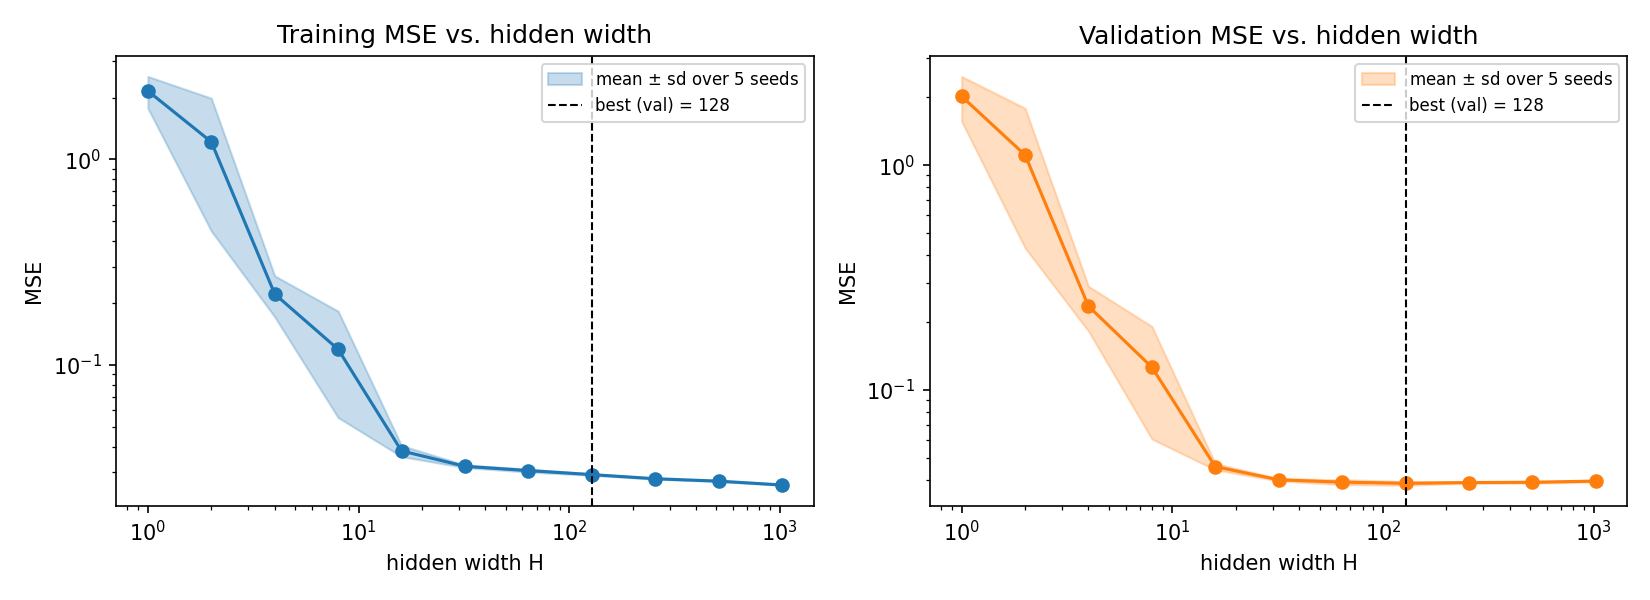
\includegraphics[width=\textwidth]{problem3_mlp_sweep.png}
\caption{MLP: training (left) and validation (right) MSE vs.\ hidden width $H$ (mean $\pm$ sd over
5 seeds; log axes).}
\label{fig:mlp}
\end{figure}

\begin{table}[H]\centering\small
\begin{tabular}{lccccccccc}
\toprule
$H$ & 1 & 2 & 4 & 8 & 16 & 32 & \textbf{128} & 512 & 1024\\
\midrule
train MSE & 2.153 & 1.217 & 0.221 & 0.119 & 0.0381 & 0.0321 & 0.0292 & 0.0272 & 0.0260\\
val MSE   & 2.023 & 1.110 & 0.236 & 0.126 & 0.0457 & 0.0399 & \textbf{0.0385} & 0.0389 & 0.0394\\
\bottomrule
\end{tabular}
\caption{Selected points of the MLP width sweep (means over 5 seeds; full results in
\texttt{problem3\_mlp\_sweep.csv}).}
\end{table}

\begin{itemize}
\item \textbf{Narrow networks underfit.} With $H\le8$ ReLU units, the function is piecewise linear
with very few pieces, which cannot represent the curved surface. Results also vary strongly with
the initialization (large error bands): with very few units, some seeds end with ``dead'' or
badly placed units.
\item From $H\approx32$ onwards the validation MSE is flat at about $0.039$. The best value is
$H^\star=128$ (validation MSE $0.0385\pm0.0008$).
\item \textbf{Very wide networks overfit only mildly.} Training MSE keeps decreasing
($0.026$ at $H=1024$, below the noise variance $\approx0.034$), so the network starts fitting
noise. Validation MSE rises only slightly ($0.0385\to0.0394$). With a fixed training budget, the
implicit regularization of (stochastic) gradient descent keeps the wide networks from
interpolating the data.
\end{itemize}

%==========================================================================
\section*{(d) Comparison and visualization}

\paragraph{Refit and validation loss.} Both models were refit on the training set with the
selected hyper-parameters (seed 0):

\begin{table}[H]\centering
\begin{tabular}{lcccc}
\toprule
Model & hyper-parameters & \# trained params & train MSE & \textbf{val MSE}\\
\midrule
Constant (train mean)    & --- & 1 & 2.463 & 2.397\\
RKS + ridge              & $\sigma=3.47$, $D=1000$, $\lambda=10^{-3}$ & 1{,}001 & 0.0333 & \textbf{0.0357}\\
1-hidden-layer MLP       & $H=128$, ReLU, Adam                     & 513     & 0.0293 & 0.0388\\
\midrule
\multicolumn{4}{l}{\emph{Reference:} least squares on $\{1,\sin x_1,x_2^2\}$ (true functional form)} & 0.0353\\
\bottomrule
\end{tabular}
\end{table}

The test-set predictions are in \texttt{rks\_test\_predictions.csv} and
\texttt{mlp\_test\_predictions.csv}, one value per row in the order of \texttt{test.csv}. The two
models agree closely on the test inputs: the mean squared difference between their predictions is
$0.0026$.

\paragraph{Which is better and why.} Both models capture the function well: about 98.5\% of the
validation variance is explained. RKS has the lower validation MSE ($0.0357$ vs.\ $0.0388$),
essentially at the noise floor ($0.0353$). With only 200 validation points, each validation MSE
has a standard error of about $0.003$ ($0.0035$ for RKS, $0.0037$ for the MLP, computed from the
per-point squared errors). The $\pm$ values in the sweep tables reflect only the randomness of the
features or the initialization, not the sampling of the validation set. Compared naively, the gap
of $0.0031$ would be only about $0.6$ (unpaired) standard errors ($0.0051$).

Both models are, however, scored on the \emph{same} validation points, and their squared errors
are highly correlated across points (correlation $0.94$): the points that are hard for one model
are hard for the other, because most of the error is the irreducible noise $\varepsilon_i$. The
right comparison is therefore paired. With $d_i=(y_i-\hat f_{\text{MLP}}(x_i))^2-(y_i-\hat
f_{\text{RKS}}(x_i))^2$,
\[
 \bar d = 0.0031,\qquad \widehat{\mathrm{SE}}(\bar d)=\frac{s_d}{\sqrt{200}}=0.0012,\qquad t\approx2.5 .
\]
On the same validation points, the paired difference is $0.0031\pm0.0012$, which \emph{is} clearly
larger than its standard error (about 2.5 SE). The gap also has the same sign for all five random
seeds of both models ($0.0031, 0.0036, 0.0026, 0.0015, 0.0027$; mean $0.0027$). So there is
reasonably good evidence that RKS fits this function slightly better, but the difference is small
in absolute terms, about $8\%$ of the MSE, and both models are close to the noise floor.

Two caveats apply. First, $\sigma^\star$ and $H^\star$ were both selected on this validation set,
so both validation MSEs are slightly optimistic. Both validation curves are very flat near their
minima (Figures~\ref{fig:rks} and~\ref{fig:mlp}), so the selection bias should be small and
similar for the two models. Second, the noise-floor reference ($0.0353$) is estimated on the same
200 points and has a similar standard error, so ``at the noise floor'' should be read as ``not
distinguishable from it''.

Plausible reasons why RKS comes out slightly ahead are:
\begin{enumerate}
\item \textbf{Right inductive bias.} RKS with $\sigma=3.47$ approximates a Gaussian-kernel ridge
regression whose function class consists of very smooth (infinitely differentiable) functions.
The true function $\sin x_1+\tfrac12x_2^2$ is exactly of this kind: smooth, low-frequency, and
without kinks. A ReLU network is \emph{piecewise linear}. It has to approximate curvature with
many flat pieces joined at kinks, and with only 600 noisy points some kinks end up in the wrong
place.
\item \textbf{Convex, closed-form fit.} The random features are fixed, so ridge regression gives
the exact global optimum, and its regularization ($\lambda$, $\sigma$) is explicit and easy to
tune. The MLP solves a non-convex problem with SGD noise. Its effective regularization comes
implicitly from the optimizer and training length, and its training MSE ($0.029$) is already below
the noise variance, i.e.\ it fits some noise.
\item \textbf{Low dimension.} In $d=2$, 500 random directions cover all orientations densely,
and because the target is smooth, slowly varying features suffice to build it. The main advantage of the MLP, \emph{learning} which features to use,
matters most in high dimensions or for functions with localized or non-smooth structure, and
neither is the case here.
\end{enumerate}
The MLP's strengths show up in other ways: it reaches nearly the same accuracy with about half as
many trained parameters (513 vs.\ 1001), and its accuracy is insensitive to the width once
$H\ge32$, while RKS fails badly for $\sigma$ that is too small.

\paragraph{Fitted surfaces.}
Figures~\ref{fig:rks_surf} and~\ref{fig:mlp_surf} were made with the provided
\texttt{plot\_surface\_2d}. Figure~\ref{fig:cmp} shows the training data and both fits on a common
colour scale, together with their difference.

\begin{figure}[H]\centering
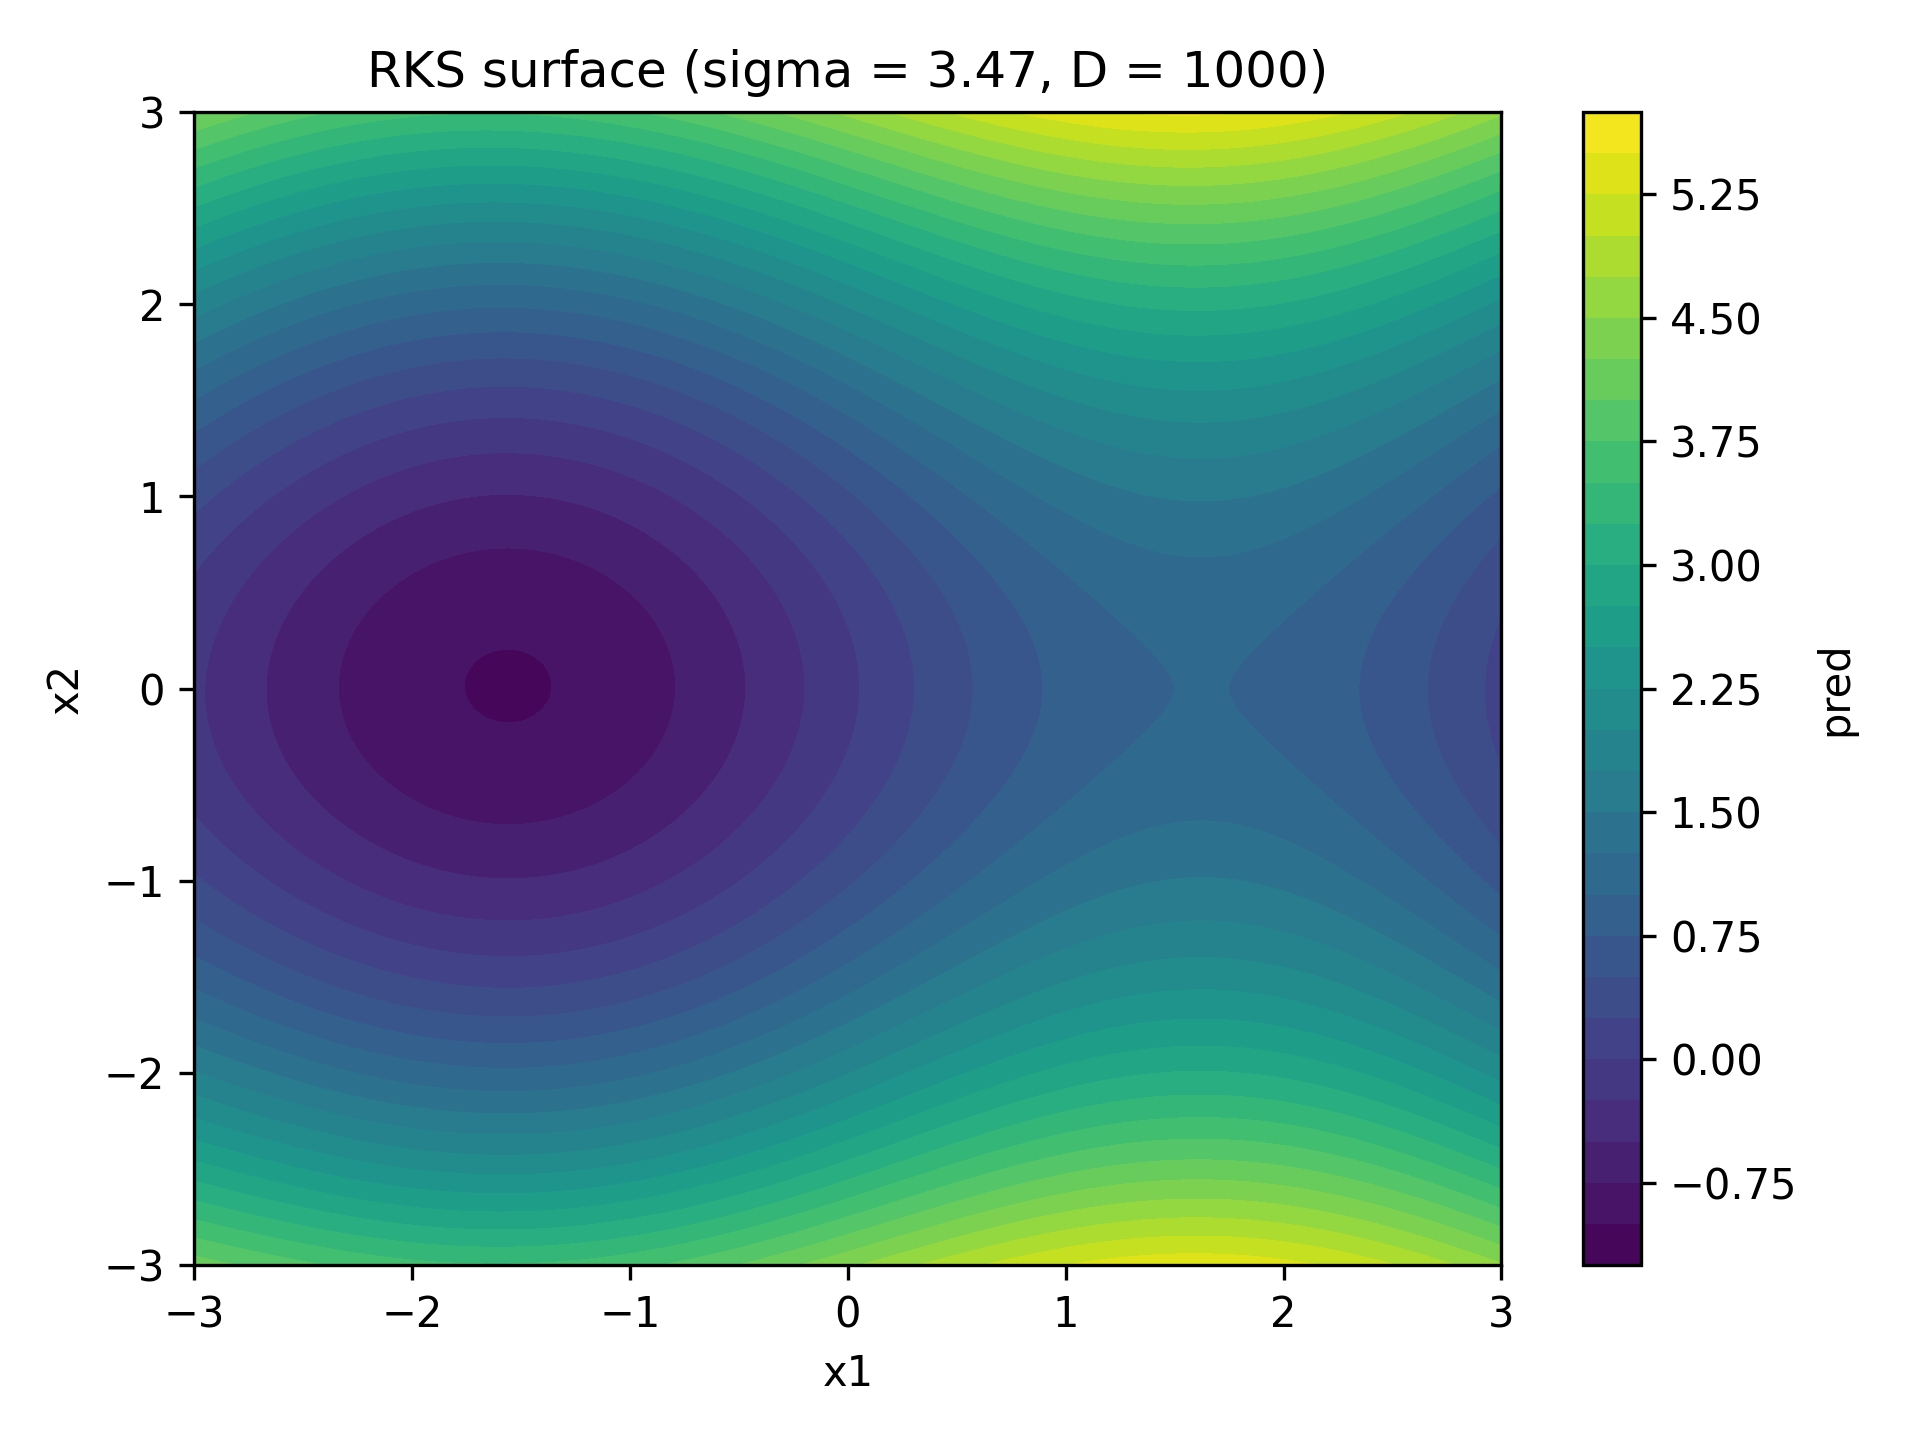
\includegraphics[width=0.48\textwidth]{problem3_rks_surface.png}\hfill
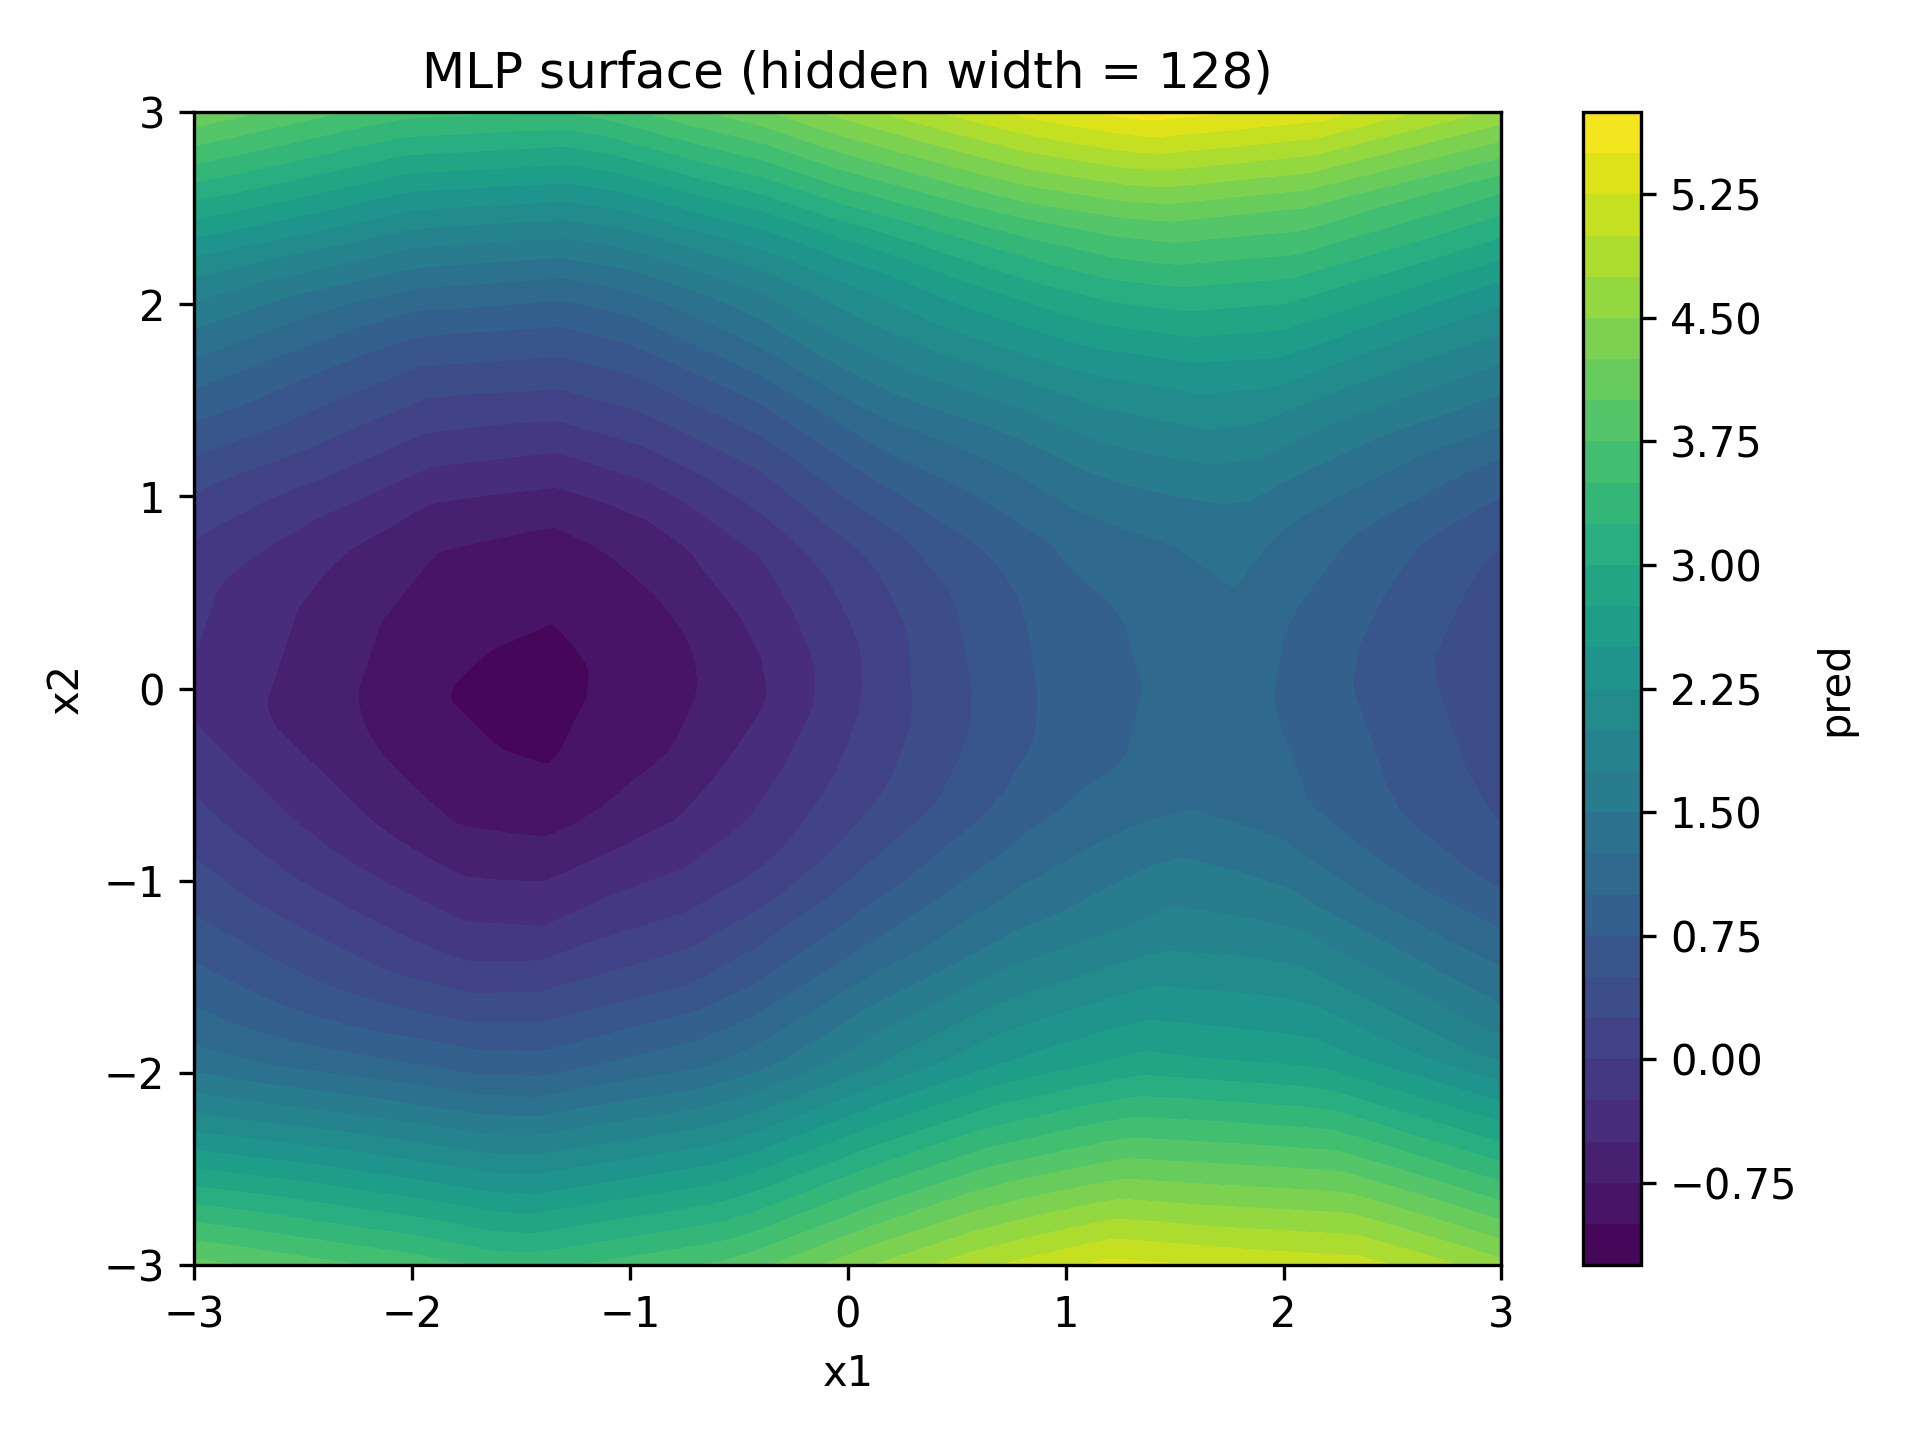
\includegraphics[width=0.48\textwidth]{problem3_mlp_surface.png}
\caption{Fitted surfaces from \texttt{plot\_surface\_2d}. Left: RKS ($\sigma=3.47$). Right: MLP
($H=128$).}
\label{fig:rks_surf}\label{fig:mlp_surf}
\end{figure}

\begin{figure}[H]\centering
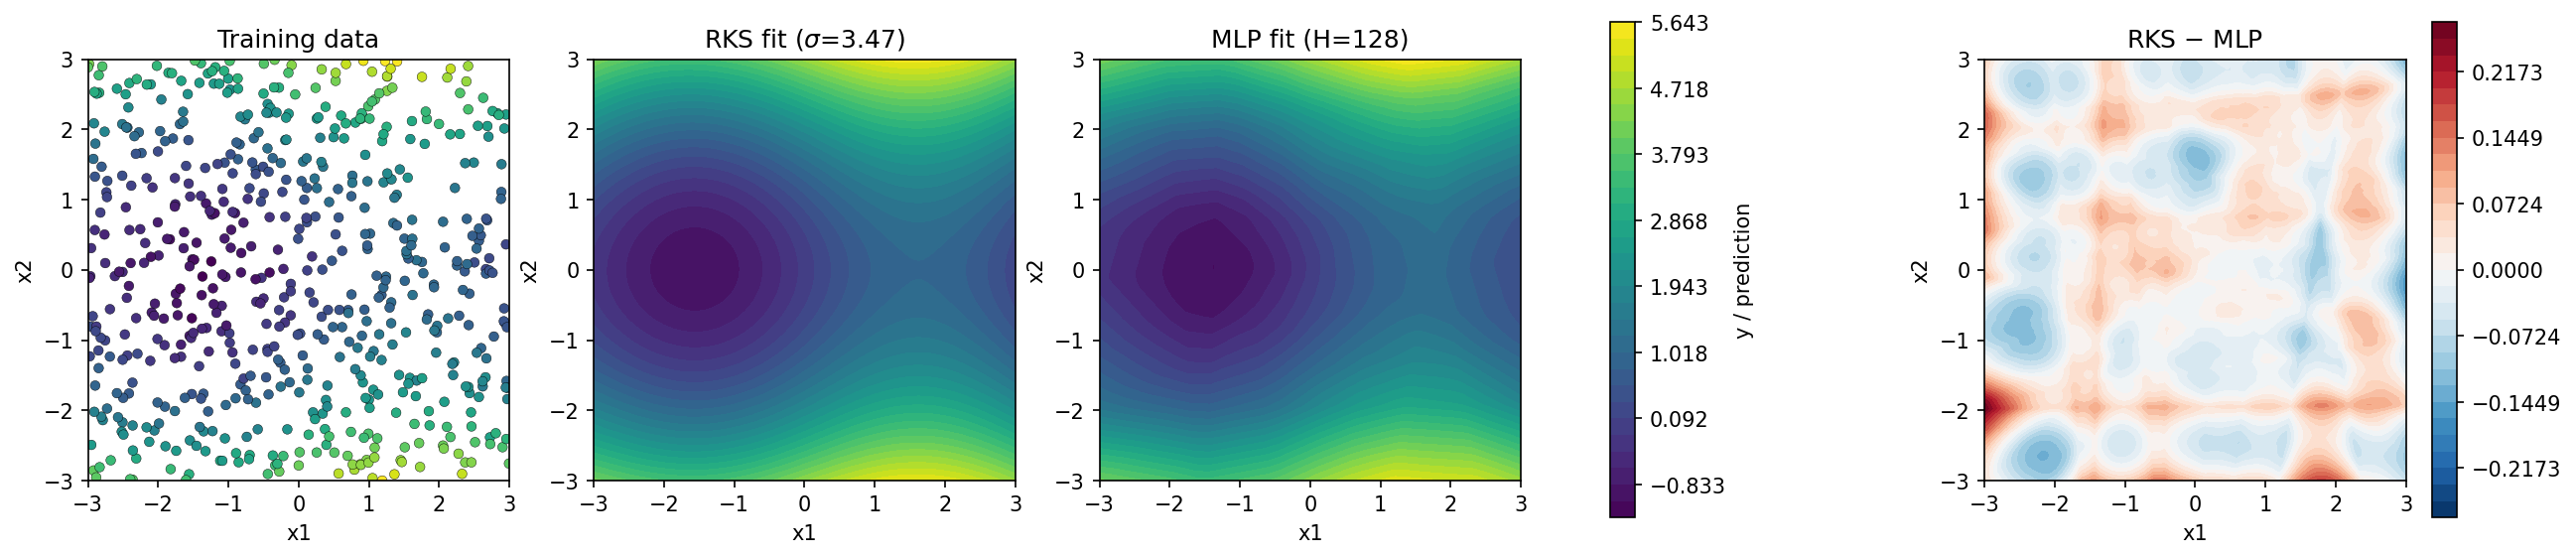
\includegraphics[width=\textwidth]{problem3_comparison.png}
\caption{From left to right: training data; RKS fit; MLP fit (shared colour scale); pointwise
difference RKS $-$ MLP.}
\label{fig:cmp}
\end{figure}

\paragraph{How each model captures the structure.} Compared with the data in (a), both surfaces
reproduce the global structure: the valley at $(x_1,x_2)\approx(-\pi/2,0)$, the ridge along
$x_1\approx\pi/2$, the symmetric parabolic growth in $|x_2|$, and the maxima in the corners
$(\pi/2,\pm3)$. The surfaces are much smoother than the triangulated data in
Figure~\ref{fig:data}, i.e.\ both models average out the observation noise instead of chasing
individual points. The two models differ only in the details:
\begin{itemize}
\item The \textbf{RKS} surface is a weighted sum of 1000 smooth sinusoids. At $\sigma^\star=3.47$
their typical wavelength $2\pi/\lVert w_j\rVert$ is about $17$, much longer than the width of the
domain. Since $\sigma\lVert w_j\rVert$ is Rayleigh-distributed in $d=2$, only a fraction
$P(\lVert w_j\rVert\ge1)=e^{-\sigma^2/2}\approx0.25\%$ of the features (about one of the 500
frequencies) oscillates at least as fast as $\sin x_1$. The oscillation in $x_1$ is therefore not
copied from any single feature but built by combining many slowly varying ones, which is why the
level sets are smooth, rounded curves, as expected for a Gaussian-kernel smoother.
\item The \textbf{MLP} surface is a sum of 128 ReLU ``hinges''. Each one is linear on either
side of a line $w_k^\top x+c_k=0$. Its contours are made of nearly straight segments with slight
corners. This is clearest in the valley, which comes out more polygonal (diamond-shaped) than
round, and in the difference plot (right panel of Figure~\ref{fig:cmp}), which shows
straight-line artefacts along the learned hinge directions.
\item The two fits differ by at most about $0.3$, and the largest differences are at the
\textbf{edges and corners} of the square (e.g.\ near $(-3,-2)$), where data are sparse and each
model extrapolates according to its own inductive bias. A ReLU network continues linearly, while
the RKS fit continues smoothly. In the interior, where the data are dense, the differences are
mostly below $0.1$, well under the noise standard deviation ($\approx0.18$).
\end{itemize}

\end{document}
